\section{Implementação}
Antes de começarmos a implementar a aplicação, decidimos estabelecer primeiro os dados do programa, isto é, os componentes e pacotes existentes, bem como as incompatibilidades e complementaridades entre si.

No que toca a componentes, dividimo-los em seis tipos, com as seguintes especificações:
\begin{enumerate}
    \item Pintura \begin{itemize} \item Cinzento \item Branco \item Preto \end{itemize}
    \item Jantes \begin{itemize} \item 19" \item 20" \item 21" \end{itemize}
    \item Pneus \begin{itemize} \item Normal \item Largo \item XL \item Off-road \end{itemize}
    \item Motorização \begin{itemize} \item 1.0 \item 1.4 \item 1.6 \item 1.8 \item 2.0 \item Turbo \end{itemize}
    \item Vidros \begin{itemize} \item Normais \item Escurecidos \end{itemize}
    \item Estofos \begin{itemize} \item Tecido - Cinzentos \item Tecido - Pretos \item Pele - Castanhos \item Pele - Pretos \end{itemize}
\end{enumerate}

Relativamente às relações, definimos que todos os componentes dum mesmo tipo são incompatíveis entre si. Além dessas incompatibilidades, escolhemos incompatibilizar as jantes 19" com os pneus XL e Off-road, bem como a motorização Turbo com as jantes 19" e os pneus Normais. Porém, existem também relações de complementaridade, como foi referido anteriormente. Estas dizem respeito ao seguinte: a jante 19" precisa de um pneu Normal, o pneu XL precisa de uma jante 20", o pneu Off-road precisa de uma jante 21" e a motorização Turbo necessita de um pneu XL.

No que toca aos pacotes, definimos também seis: o \textit{Sport}, o \textit{Comfort}, \textit{Off-road}, \textit{Executive}, \textit{Classic} e \textit{Economic}.

Os componentes englobados em cada pacote são os seguintes:
\begin{enumerate}
    \item \textit{Sport}: Jantes 20", Pneus XL, Motorização Turbo e Estodos de Tecido Pretos
    \item \textit{Comfort}: Pintura Cinzenta, Pneus Largos e Estofos de Tecido Cinzentos
    \item \textit{Off-road}: Jantes 21", Pneus Off-road e Motorização 2.0
    \item \textit{Executive}: Pintura Preta, Motorização 1.8, Vidros Escurecidos e Estofos de Pele Pretos
    \item \textit{Classic}: Pintura Branca, Jantes 19", Motorização 1.0 e Estofos de Pele Castanhos
    \item \textit{Economic}: Jantes 20" e Motorização 1.4.
\end{enumerate}


\subsection{Algoritmo de Configuração ótima}
Uma das funcionalidades propostas permite o calculo automático de uma configuração quando dado um orçamento. O nosso algoritmo para o calculo da mesma é descrito da seguinte maneira:
\begin{enumerate}
    \item Usando uma lista com todos os componentes, construimos a lista prim com apenas os componentes com dependências e a lista sng com componentes sem dependências.
    \item Ordenamos a lista prim pela razão entre o custo total (custo componente + custo das dependências) e o número de componentes que são adicionados. (heuristica da razão)
    \item Ordenamos a lista sng pelo custo.
    \item Iteramos a lista prim e adicionamos o componente à configuração se for possível adicionar todas as suas dependências sem que o orçamento seja ultrapassado ou que a configuração tenha incompatibilidades.
    \item Por fim iteramos a lista sng e, se for possível, adicionamos o componente à configuração.
\end{enumerate}

Este algoritmo construi uma configuração válida e dentro do orçamento.

\newpage
\subsection{Base de dados implementada}
Ao transformar o diagrama de classes num diagrama com ORM foi necessário que algumas classes passassem a persistir e, para tal, implementamos um sistema de dados MySQL. De seguida é apresentado o modelo lógica do mesmo:

\begin{center}
 	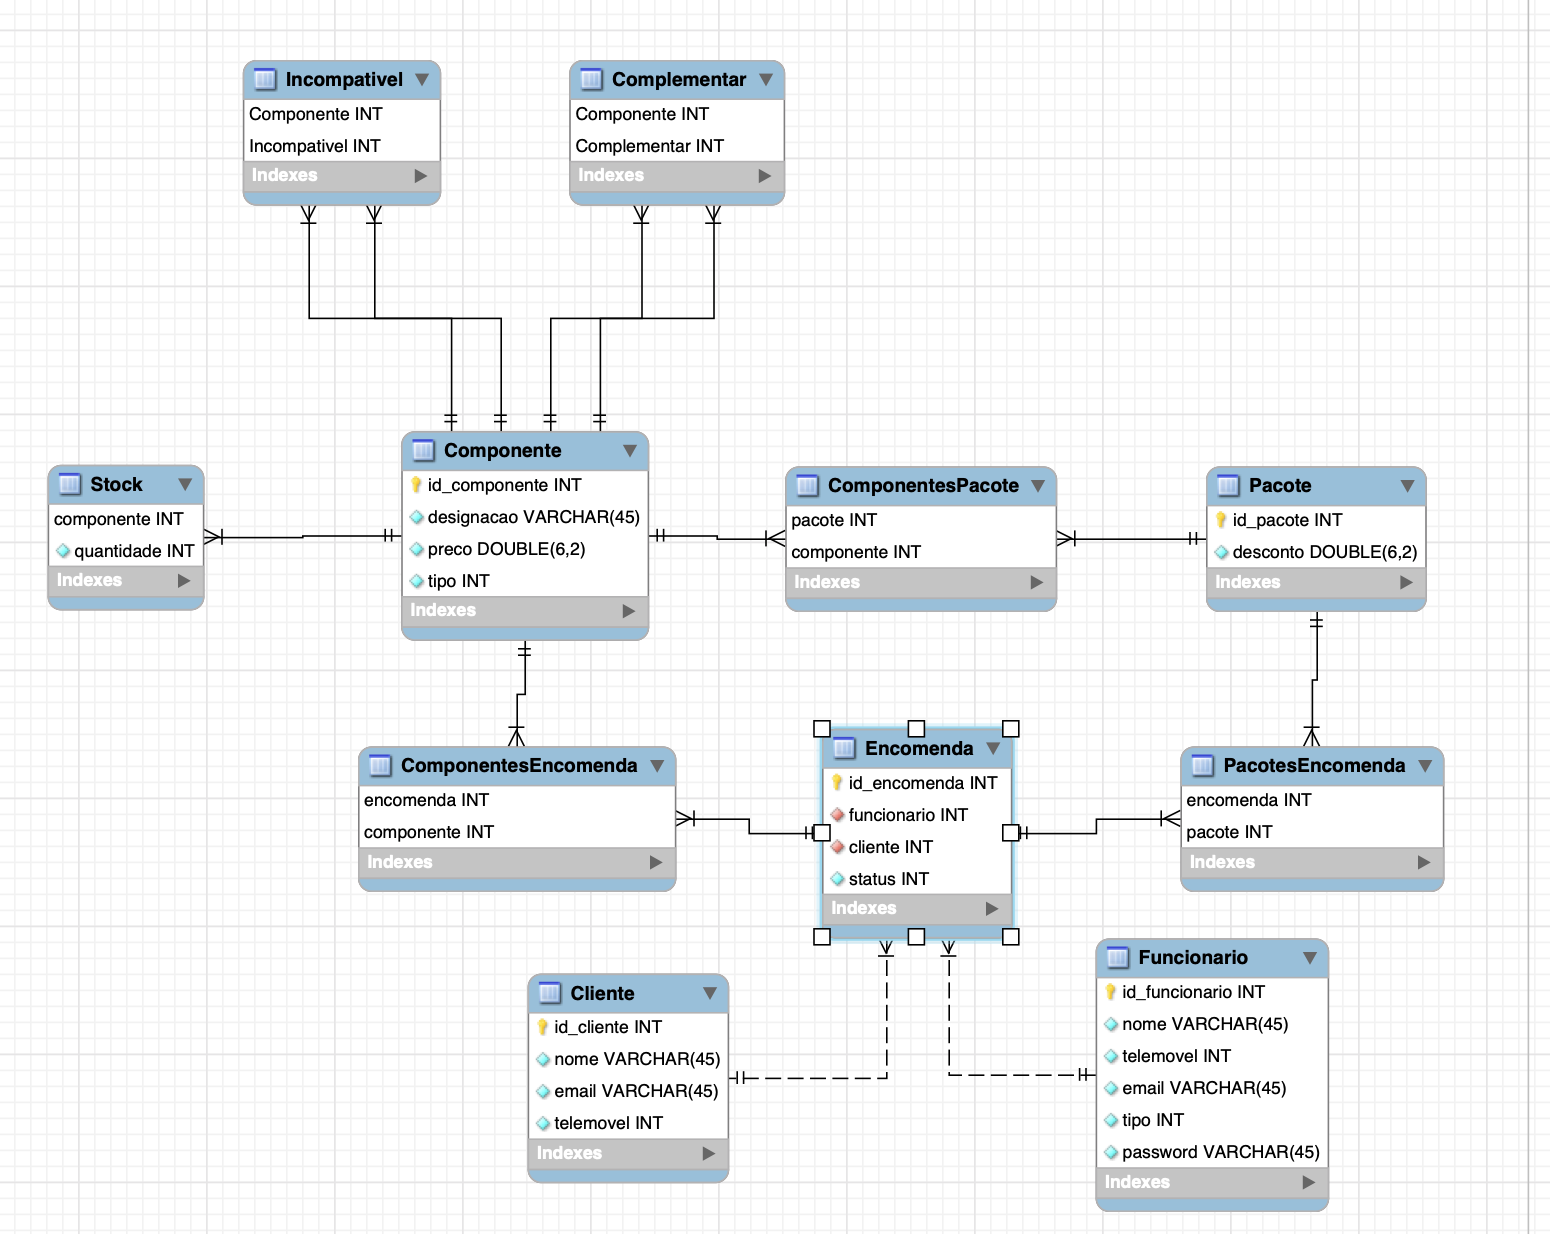
\includegraphics[width = 5.5in]{VPP/modelologico.png}
\end{center}
\newpage